

General equation of the circle in vector form is :
\begin{align}
\vec{x}^T\vec{x}+2\vec{u}^T\vec{x}+f=0\label{eq:solutions/18/1/eq:1}
\end{align}
In the vector form \eqref{eq:solutions/18/1/eq:0} can be written as :
\begin{align}
\vec{x}^T\vec{x}+2\myvec{\frac{-3}{2}\\[0.1 cm]5}^T\vec{x}-15=0\label{eq:solutions/18/1/eq:2}
\end{align}
By comparing \eqref{eq:solutions/18/1/eq:1} and \eqref{eq:solutions/18/1/eq:2} we get : 
\begin{align}
    \vec{u}=\myvec{-\frac{3}{2}\\[0.1 cm]5},f=-15\label{eq:solutions/18/1/eq:3}
\end{align}
We know that the equation of tangent in the form of normal vector $(\vec{p}+\vec{u})$ and point $\vec{p}$ can be written as:
\begin{align}
    (\vec{p}+\vec{u})^T(\vec{x}-\vec{p})&=0\\
    (\vec{p}+\vec{u})^T\vec{x}-\vec{p}^T\vec{p}-\vec{u}^T\vec{q}&=0\label{eq:solutions/18/1/eq:5}
\end{align}
Using \eqref{eq:solutions/18/1/eq:1}, \eqref{eq:solutions/18/1/eq:5} will become : 
\begin{align}
    (\vec{p}+\vec{u})^T\vec{x}+\vec{u}^T\vec{p}+f&=0\label{eq:solutions/18/1/eq:6}
\end{align}
By putting the values of $\vec{p}$, $\vec{u}$ and $f$ from \eqref{eq:solutions/18/1/eq:3} in \eqref{eq:solutions/18/1/eq:6} we get : 
\begin{align}
    \myvec{\frac{5}{2}&-6}\vec{x}+\myvec{4&-11}\myvec{\frac{-3}{2}\\[0.2cm]5}-15&=0\\
    \myvec{\frac{5}{2}&-6}\vec{x}-76&=0
\end{align}
Hence the equation of the tangent to the circle passing through the point $\vec{p}$ is:
\begin{align}
    \myvec{\frac{5}{2}&-6}\vec{x}&=76\label{eq:solutions/18/1/eq:9}
\end{align}
Plot of the tangent to a circle given by equation \eqref{eq:solutions/18/1/eq:9} is as follows :
\begin{figure}[h]
\centering
    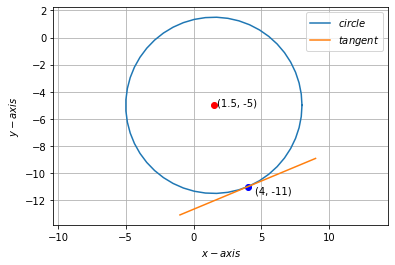
\includegraphics[width=\columnwidth]{solutions/18/1/tangent.png}
    \caption{Tangent to a circle centered at $(1.5, -5)$ with radius $6.5$ passing through the point $(4,-11)$.}
    \label{eq:solutions/18/1/tangent}
\end{figure}

